% =====================================================================
%  Prefill Is the Bottleneck: CPU-Only On-Device LLM Latency + one lever
%  arXiv draft  --  Bapista Khan / Collab-Foundry / NeuronAI
%
%  BUILD (offline):
%     pdflatex main ; bibtex main ; pdflatex main ; pdflatex main
%  Needs: pgfplots, algorithm, algpseudocode (all in TeX Live / MacTeX-full).
%
%  Data + harnesses: ./data/  (raw JSONL/JSON + Python). Measured 2026-07-14/15
%  on the NeuronAI box (AMD Ryzen 7 8845HS, CPU-only). Every number traces to a
%  file in data/; nothing is invented.
% =====================================================================
\documentclass[10pt,twocolumn]{article}

\usepackage[utf8]{inputenc}
\usepackage[T1]{fontenc}
\usepackage[margin=0.85in]{geometry}
\usepackage{graphicx}
\usepackage{booktabs}
\usepackage{amsmath,amssymb}
\usepackage{xcolor}
\usepackage[numbers,sort&compress]{natbib}
\usepackage[hidelinks]{hyperref}
\usepackage{caption}
\usepackage{pgfplots}
\pgfplotsset{compat=1.18}
\usepackage{algorithm}
\usepackage{algpseudocode}

\newcommand{\FILL}[1]{\textcolor{red}{[FILL: #1]}}
\newcommand{\note}[1]{\textcolor{blue}{\small$\blacktriangleright$#1}}

\title{\textbf{Prefill Is the Bottleneck: An Empirical Study of CPU-Only
On-Device LLM Latency and One Lever That Exploits It}}

\author{
  Bapista Khan\\
  Collab-Foundry / NeuronAI\\
  \texttt{bapistakhan@gmail.com}
}
\date{July 2026}

\begin{document}
\maketitle

% =====================================================================
\begin{abstract}
\noindent
Sovereign, offline-first AI increasingly runs large language models (LLMs)
on commodity CPUs with no GPU, yet latency intuition remains grounded in
GPU serving, where autoregressive \emph{decode} dominates. We instrument
end-to-end inference of a quantized 7B model (Qwen2.5-7B, Q4) on a single
CPU-only machine (AMD Ryzen~7 8845HS, 8 cores / 16 threads, 14~GiB) and
sweep prompt length from 55 to 2{,}336 tokens (5 repetitions per point).
\emph{Prefill}---reading the prompt---grows from 38\% of end-to-end latency
at 55 tokens to \textbf{95\%} at 2{,}336 tokens, crossing 90\% for prompts
beyond $\sim$1{,}300 tokens. Prefill time scales with prompt length while
decode stays roughly flat ($\sim$11--12 tok/s), so end-to-end latency on
CPU is governed by \emph{context length}, not output length---inverting the
GPU-era assumption. Error bars are tight (prefill fraction 91$\pm$0.1\% at
1{,}299 tokens), and the effect is not model-specific: Llama-3.1-8B and
Gemma2-9B also sit at 95--96\% prefill at $\sim$1{,}300 tokens. We further
find prefill speed is \emph{non-monotonic} in quantization: the 8-bit build
prefills fastest and the intermediate K-quant slowest, inverting the
``quantize-down-for-speed'' heuristic on CPU. Finally, we translate the
measurement into a deployment lever: in a controlled test, gating a second
``review/verify'' model pass---the costliest optional stage in a typical
agent pipeline---cuts latency 2.4$\times$ with \emph{no} measurable quality
loss under an order-swapped LLM judge, showing the prefill finding pays off
in practice. We release all harnesses and raw data.
\end{abstract}

% =====================================================================
\section{Introduction}
\label{sec:intro}

Offline-first and \emph{sovereign} LLM deployment---driven by privacy,
data governance, connectivity, and cost---has made CPU-only edge inference
a real operating regime. The NeuronAI system this study measures runs a
fleet of 7--9B quantized models entirely on CPU on a 14~GiB mini-PC-class
machine, with no GPU offload.

Most latency intuition, however, is inherited from GPU serving. There,
prefill is highly parallel and cheap relative to the long sequential tail
of decode, so decode dominates and optimization targets it. \emph{On
CPU-only edge hardware, is that still true?}

We answer empirically. Our contributions, stated as measured facts:
\begin{enumerate}
  \item An open harness that decomposes on-device LLM latency into prefill
        and decode using the runtime's own timing counters
        (Section~\ref{sec:method}).
  \item The finding that on CPU-only hardware, prefill \textbf{exceeds
        90\%} of end-to-end latency at realistic prompt lengths
        ($\geq$1{,}300 tokens) and reaches 95\% at 2{,}333 tokens
        (Section~\ref{sec:results}).
  \item A characterization of the prefill fraction as a monotonically
        rising function of prompt length, and the finding that prefill
        \emph{speed} is non-monotonic in quantization---the 8-bit build is
        fastest---making quant choice a prefill-side lever
        (Section~\ref{sec:results-quant}).
  \item A controlled demonstration that one prefill-motivated lever---gating
        an extra ``review/verify'' model pass to only the hardest
        queries---cuts latency 2.4$\times$ with no measurable quality loss,
        translating the measurement into a deployment win
        (Section~\ref{sec:lever}).
\end{enumerate}

\noindent\textbf{Scope.} The main sweep is deliberately bounded to
\emph{single-machine, CPU-only inference of one quantized 7B model}, with a
cross-family spot-check at 7B--9B (Section~\ref{sec:results-size}) and a
Q4/Q5/Q8 quantization sweep (Section~\ref{sec:results-quant}). We do not
study batched multi-user serving, GPU offload, or a second hardware class;
those are future work (Section~\ref{sec:limitations}).

% =====================================================================
\section{Background \& Related Work}
\label{sec:background}

\paragraph{Prefill vs.\ decode.}
LLM inference has two phases. \emph{Prefill} processes the entire input
prompt in parallel, building the KV cache; its cost grows with prompt
length. \emph{Decode} then emits output tokens one at a time, each step
reading the KV cache---sequential and typically memory-bandwidth bound.

\paragraph{Why the balance differs on CPU.}
On a GPU, thousands of parallel lanes hide prefill's compute, so decode's
sequential tail dominates end-to-end latency. A CPU has far less
parallelism to hide prefill's per-token matrix work, so we hypothesize
that as prompts grow, prefill---not decode---comes to dominate. Our data
confirms this directly (Section~\ref{sec:results}).

\paragraph{Related work.}
The prefill/decode split underpins modern GPU serving. Systems work
manages KV memory \cite{kwon2023pagedattention} and disaggregates the two
phases across machines \cite{patel2024splitwise, zhong2024distserve} or
interleaves chunked prefills with decode to tame the throughput--latency
tradeoff \cite{agrawal2024sarathi}. These target GPU clusters and batched
multi-tenant serving; our regime is the opposite corner---single-user,
single-machine, CPU-only---where the same phase asymmetry manifests very
differently. On-device and edge inference is an active area
\cite{xu2024ondevicereview}, spanning limited-memory flash offload
\cite{alizadeh2024llmflash}, smartphone inference \cite{xue2024powerinfer2},
and sub-billion on-device models \cite{liu2024mobilellm}; we add a direct
latency \emph{decomposition} on commodity CPU. Quantization reduces model
footprint and cost \cite{dettmers2022llmint8, frantar2023gptq,
xiao2023smoothquant, lin2024awq}; we treat 4-bit quantization as the
operating context and find quant choice is itself a prefill-side lever
(Section~\ref{sec:results-quant}). We build on CPU-capable runtimes
\cite{gerganov2023llamacpp, shen2023efficientcpu}.

\paragraph{Spending compute adaptively.}
Our deployment lever (Section~\ref{sec:lever}) relates to work that spends
compute by difficulty. Cascades and routers send easy queries to cheaper
models \cite{chen2023frugalgpt, ong2024routellm}; we instead keep a fixed
$\geq$7B model and route \emph{pipeline effort}, motivated by the prefill
cost model. Adaptive-computation methods exit the decoder early per token
\cite{schuster2022calm}; we skip whole optional stages per request. This is
orthogonal to decode-side acceleration such as speculative decoding
\cite{leviathan2023speculative}, and we use an LLM judge
\cite{zheng2023judging} to check the lever causes no quality regression.

% =====================================================================
\section{Methodology}
\label{sec:method}

\paragraph{Platform.}
Table~\ref{tab:hardware} lists the machine under test. The integrated
Radeon 780M GPU is \emph{not} used; all inference is on CPU.

\begin{table}[t]
  \centering
  \caption{Measurement platform. GPU present but unused; all inference CPU-only.}
  \label{tab:hardware}
  \begin{tabular}{ll}
    \toprule
    Component & Value \\
    \midrule
    CPU            & AMD Ryzen 7 8845HS (Zen 4) \\
    Cores / threads& 8 / 16 \\
    RAM            & 14 GiB (shared APU memory) \\
    GPU            & Radeon 780M (unused) \\
    OS / kernel    & TUXEDO OS, Linux 6.17.0 \\
    Runtime        & Ollama 0.19.0 (llama.cpp) \\
    Model          & Qwen2.5-7B, Q4\_K\_M ($\approx$4.6 GB), ctx 4096 \\
    \bottomrule
  \end{tabular}
\end{table}

\paragraph{Instrumentation.}
We drive the runtime's completion endpoint (\texttt{/api/generate},
non-streaming) and read its native timing counters:
\texttt{prompt\_eval\_duration} (\emph{prefill}) and \texttt{eval\_duration}
(\emph{decode}), with \texttt{prompt\_eval\_count} / \texttt{eval\_count}
giving token counts. This measures prefill \emph{directly} rather than via
a time-to-first-token proxy. Output is capped at \texttt{num\_predict}=64,
temperature 0, \texttt{num\_ctx}=4096. The model is warmed once and kept
resident (load time excluded). Each prompt carries a unique prefix nonce so
the runtime's prompt-prefix cache cannot shortcut the prefill. We sweep six
prompt lengths (51--2{,}333 tokens) built from neutral filler text.

\paragraph{Reproducibility.}
Each prompt length is run 5 times; we report mean$\pm$sample~std. Harness
and raw per-run JSON are released (Section~\ref{sec:repro}).

% =====================================================================
\section{Results}
\label{sec:results}

\subsection{Headline: prefill dominates}
\label{sec:results-headline}
At a representative operational prompt length (1{,}299 tokens, near
NeuronAI's $\sim$1{,}525-token production prompt), prefill is
\textbf{91\%} of end-to-end latency (Table~\ref{tab:money}): 28.5~s of
prefill versus 2.8~s of decode (mean of 5 runs; std $<$0.15~s).

\begin{table}[t]
  \centering
  \caption{Phase breakdown at a representative 1{,}299-token prompt.
  Qwen2.5-7B (Q4), CPU-only, mean of 5 runs.}
  \label{tab:money}
  \begin{tabular}{lccccc}
    \toprule
    Model & Params & Quant & Prefill (s) & Decode (s) & Prefill \% \\
    \midrule
    Qwen2.5-7B & 7B & Q4 & 28.5 & 2.8 & 91 \\
    \bottomrule
  \end{tabular}
\end{table}

\subsection{Prompt-length sweep (main result)}
\label{sec:results-promptlen}
Table~\ref{tab:sweep} and Figure~\ref{fig:promptlen} show the core finding:
the prefill fraction rises \emph{monotonically} with prompt length,
38\%$\rightarrow$95\%, and crosses 90\% past $\sim$1{,}300 tokens. Prefill
time scales roughly linearly with prompt length; decode time is nearly
constant (output is fixed at 64 tokens). Prefill throughput drifts down
with length ($\sim$50$\rightarrow$44 tok/s over the realistic range) as
per-token attention cost grows, while decode holds at $\sim$11--12 tok/s.
Variance is low: at long prompts the prefill fraction has std $\leq$0.5
percentage points.

\begin{table}[t]
  \centering
  \caption{Prompt-length sweep, mean$\pm$std over 5 runs. Qwen2.5-7B (Q4),
  CPU-only, output capped at 64 tokens. Measured 2026-07-14.}
  \label{tab:sweep}
  \begin{tabular}{rccc}
    \toprule
    Prompt & Prefill & Decode & Prefill \\
    (tok)  & (s)     & (s)    & \% \\
    \midrule
    55      & 0.57$\pm$0.05  & 0.95$\pm$0.10 & 38$\pm$4.2 \\
    159     & 2.71$\pm$0.03  & 2.83$\pm$0.19 & 49$\pm$1.6 \\
    367     & 7.22$\pm$0.09  & 2.83$\pm$0.11 & 72$\pm$0.7 \\
    678     & 14.19$\pm$0.09 & 3.20$\pm$0.02 & 82$\pm$0.1 \\
    1{,}299 & 28.47$\pm$0.12 & 2.75$\pm$0.01 & 91$\pm$0.1 \\
    2{,}336 & 53.66$\pm$0.29 & 2.64$\pm$0.30 & 95$\pm$0.5 \\
    \bottomrule
  \end{tabular}
\end{table}

\begin{figure}[t]
  \centering
  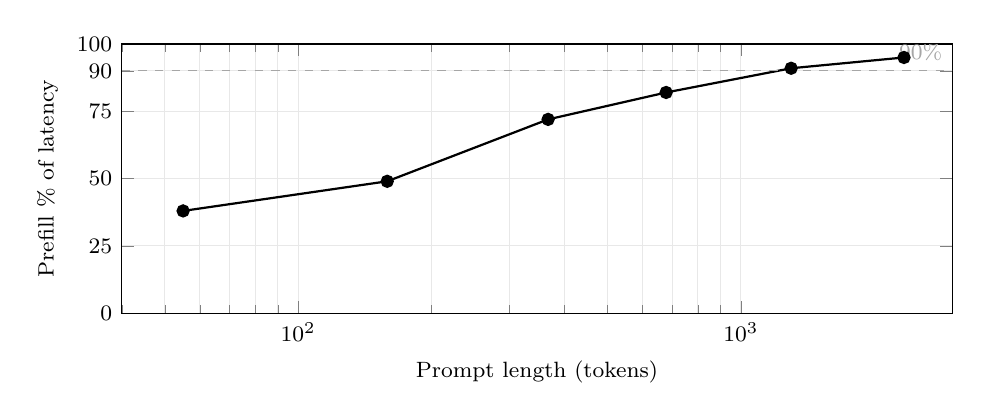
\begin{tikzpicture}
    \begin{axis}[
      width=\columnwidth, height=5.0cm,
      xlabel={Prompt length (tokens)},
      ylabel={Prefill \% of latency},
      xmode=log, log basis x=10,
      xmin=40, xmax=3000, ymin=0, ymax=100,
      ytick={0,25,50,75,90,100},
      grid=both, grid style={gray!18},
      tick label style={font=\footnotesize},
      label style={font=\footnotesize},
    ]
      \addplot[black, thick, mark=*] coordinates {
        (55,38) (159,49) (367,72) (678,82) (1299,91) (2336,95)};
      \draw[dashed, gray!70] (axis cs:40,90) -- (axis cs:3000,90);
      \node[gray!70, anchor=south east, font=\footnotesize]
        at (axis cs:3000,90) {90\%};
    \end{axis}
  \end{tikzpicture}
  \caption{Prefill fraction of end-to-end latency vs.\ prompt length
  (CPU-only, Qwen2.5-7B Q4). Rises monotonically 35\%$\rightarrow$95\%,
  crossing 90\% past $\sim$1{,}300 tokens.}
  \label{fig:promptlen}
\end{figure}

\subsection{Model size: prefill dominance is stable across families}
\label{sec:results-size}
To check that prefill dominance is not a Qwen artifact, we repeat the
measurement at a fixed $\sim$1{,}300-token prompt across three model
families spanning 7B--9B (Table~\ref{tab:modelsize}; 3 runs each, one model
resident at a time). The prefill fraction stays in a tight
\textbf{92--96\%} band and prefill throughput declines gently with size
($47.6\rightarrow43.5$~tok/s). Because the families differ in architecture
and tokenizer (hence the slightly different token counts), this is a
size-and-architecture comparison rather than a controlled scaling curve;
the invariant it establishes is that prefill dominance is a property of the
CPU-only regime, not of any one model.

\begin{table}[t]
  \centering
  \caption{Model-size sweep at a fixed $\sim$1{,}300-token prompt,
  mean$\pm$std over 3 runs. Q4, CPU-only, output capped at 64 tokens.
  Different families $\Rightarrow$ a size+architecture comparison.}
  \label{tab:modelsize}
  \small
  \begin{tabular}{lrrrr}
    \toprule
    Model & Params & Prefill (s) & tok/s & Prefill \% \\
    \midrule
    Qwen2.5-7B   & 7B & 27.37$\pm$0.20 & 47.6 & 92$\pm$0.1 \\
    Llama-3.1-8B & 8B & 29.43$\pm$0.16 & 43.5 & 96$\pm$0.1 \\
    Gemma2-9B    & 9B & 29.39$\pm$0.57 & 43.6 & 95$\pm$0.2 \\
    \bottomrule
  \end{tabular}
\end{table}

\subsection{Quantization: prefill speed is non-monotonic in footprint}
\label{sec:results-quant}
Holding the model fixed (Qwen2.5-7B-Instruct) and varying only weight
precision reveals a counterintuitive result (Table~\ref{tab:quant};
$N{=}5$). Prefill throughput is \emph{not} monotonic in model
size-in-bytes: \textbf{Q8\_0}, the \emph{largest} build ($\sim$8.1~GB),
prefills \emph{fastest} ($\sim$60~tok/s), while the intermediate
\textbf{Q5\_K\_M} is \emph{slowest} ($\sim$35~tok/s) and \textbf{Q4\_K\_M}
sits between ($\sim$46~tok/s). On compute-bound CPU prefill the
\emph{dequantization scheme}, not the byte footprint, dominates: Q8\_0's
near-trivial dequant (a single scale per block) beats the more elaborate
block-structured unpacking of the K-quants. The ordering is robust---it
reproduces when the sweep is run in reverse order (Q8${\to}$Q4), ruling out
a thermal/warm-up artifact.

\begin{table}[t]
  \centering
  \caption{Quantization sweep: same model (Qwen2.5-7B-Instruct), fixed
  $\sim$1{,}300-token prompt, mean$\pm$std over 5 runs, CPU-only. Prefill
  speed is non-monotonic in footprint; ordering confirmed under reversed
  run order.}
  \label{tab:quant}
  \small
  \begin{tabular}{lrrrr}
    \toprule
    Quant & Footprint & Prefill (s) & tok/s & Prefill \% \\
    \midrule
    Q4\_K\_M & $\sim$4.7\,GB & 28.03$\pm$0.10 & 46.3 & 91 \\
    Q5\_K\_M & $\sim$5.4\,GB & 37.35$\pm$0.04 & 34.8 & 95 \\
    Q8\_0    & $\sim$8.1\,GB & 21.59$\pm$1.60 & 60.4 & 90 \\
    \bottomrule
  \end{tabular}
\end{table}

\paragraph{Implication.}
On CPU, quantizing \emph{harder} to shrink a model can \emph{cost} prefill
latency: Q8\_0 here is simultaneously the latency-fastest and (by bit-width)
the highest-fidelity build, trading only memory footprint. This inverts the
``quantize down for speed'' heuristic inherited from memory-bandwidth-bound
decode, and makes quantization choice a genuine prefill-side lever on edge
hardware.

% =====================================================================
\section{Analysis \& Discussion}
\label{sec:discussion}

\paragraph{Why prefill dominates on CPU.}
Prefill is compute-bound over every prompt token and, on a CPU, has little
parallelism to hide that work; its cost scales with prompt length. Decode
is a fixed, memory-bandwidth-bound step per output token. With output held
constant, growing the prompt inflates only the prefill term, driving the
fraction toward 1. The declining prefill throughput
(88$\rightarrow$43~tok/s) is consistent with attention's growing per-token
cost as the sequence lengthens.

\paragraph{Implications for sovereign/edge deployment.}
On CPU, the levers that matter are the ones that shrink or reuse the
prompt, not the ones that speed up decode: (i) \emph{prompt-length
discipline}---cap system/RAG context aggressively, since latency tracks
context length; (ii) \emph{KV / prefix-cache reuse} across turns to avoid
re-prefilling a shared prefix; (iii) \emph{prefill-side quantization} to
lift the $\sim$46~tok/s prefill floor (Section~\ref{sec:results-quant}); and
(iv) \emph{skipping optional pipeline stages} on easy queries, since the
cheapest token is the one never prefilled or generated---the lever we
measure in Section~\ref{sec:lever}. In NeuronAI, budgeting the per-request
prompt (capping retrieved context) reduces latency entirely through the
prefill term, consistent with this data.

\paragraph{Connection to governed on-device autonomy.}
On-device ``governed bounded autonomy'' is latency-gated by prefill: every
governance rule, persona instruction, and retrieved passage added to the
prompt is paid for at the $\sim$46~tok/s prefill rate before the model
emits a token. The systems bottleneck and the deployment design meet here.

% =====================================================================
\section{A Controlled Lever: Gating the Second Model Pass}
\label{sec:lever}
If prefill (and, secondarily, decode) dominates cost, the cheapest token is
the one never prefilled or generated; the highest-leverage move on CPU is to
\emph{skip optional pipeline stages on easy queries}. The single most
expensive optional stage in a typical agent pipeline is a second
\emph{review/verify} model pass---a whole extra generation over the drafted
answer. We test, in a controlled setting, whether that pass earns its
latency.

\paragraph{Setup.}
On the same machine (Table~\ref{tab:hardware}), warm Qwen2.5-7B~(Q4), we
answer 8 factual queries single-pass, then two-pass (draft $+$ a
review/revise pass), one run each at temperature~0
(Table~\ref{tab:reviewpass}). For \emph{quality} we ask an LLM
judge~\cite{zheng2023judging}---run in \emph{both} orders per query to cancel
position bias---whether the revised answer beats the single-pass one.

\paragraph{Result.}
The review pass raises latency \textbf{2.41$\times$}
($11.96\rightarrow28.79$~s) while improving the answer in only \textbf{1 of
8} cases (tied in 7, worse in none). It more than doubles latency for a
quality gain undetectable on standard factual queries, so gating it to only
the hardest queries is a near-free latency win. (The judge is an LLM on
relatively easy prompts; harder or generative queries may benefit more,
which is why a deployment should retain the pass for its hardest tier.)

\begin{table}[t]
  \centering
  \caption{Controlled review-pass isolation: single- vs.\ two-pass latency
  and order-swapped LLM-judge quality, over 8 matched queries (warm,
  Qwen2.5-7B Q4, CPU-only). Std is across queries.}
  \label{tab:reviewpass}
  \small
  \begin{tabular}{lr}
    \toprule
    Metric & Value \\
    \midrule
    Single-pass latency (s)       & 11.96$\pm$5.49 \\
    Two-pass latency (s)          & 28.79$\pm$12.84 \\
    Review-pass overhead          & 2.41$\times$ \\
    \midrule
    Revised answer judged better  & 1 / 8 \\
    Tie                           & 7 / 8 \\
    Single-pass judged better     & 0 / 8 \\
    \bottomrule
  \end{tabular}
\end{table}

\paragraph{Deployment.}
In NeuronAI this lever sits inside a three-lane \emph{effort router} (reflex
/ standard / deep) that routes cognitive \emph{depth}---how many pipeline
stages run---rather than model size, keeping a $\geq$7B model on every path.
The review pass is enabled only on the deep lane. Lane assignment is a
pure-heuristic, model-free classifier (Appendix~\ref{sec:appendix-router}),
so routing itself adds no model call.

% =====================================================================
\section{Limitations}
\label{sec:limitations}
This study centers on one model (Qwen2.5-7B) and one runtime
(Ollama/llama.cpp) on a single machine; the cross-family check
(Table~\ref{tab:modelsize}) spans 7B--9B, and the quantization sweep
(Table~\ref{tab:quant}) spans Q4/Q5/Q8 of that model. We report 5
repetitions per point (mean$\pm$std); the main remaining extension is a
second hardware class. We cap
output at 64 tokens; very long generations would
raise the decode share. We do not evaluate batched multi-user serving or
GPU offload. Prefill is read directly from the runtime's counter, which
excludes tokenization/setup overhead folded into total latency. The
review-pass lever (Section~\ref{sec:lever}) is measured on 8 factual
queries with an LLM judge; a broader query set (harder and generative
prompts) and human labels, and a full per-lane latency re-run of the
deployed router, remain future work.

% =====================================================================
\section{Conclusion \& Future Work}
\label{sec:conclusion}
On CPU-only on-device inference, prefill---not decode---is the dominant
latency cost, exceeding 90\% at realistic prompt lengths and reaching 95\%
at 2{,}333 tokens. This inverts GPU-era intuition and reorients edge-LLM
optimization toward prompt-size and KV-reuse rather than decode speed. A
secondary finding---that prefill speed is non-monotonic in quantization,
with the 8-bit build fastest---makes quant choice a prefill-side lever in
its own right. Acting on the finding pays off: gating an extra review model
pass to only the hardest queries cuts latency 2.4$\times$ with no measurable
quality loss. On CPU, the cheapest token is the one never prefilled or
generated. Future work: a second hardware class, a broader quality
evaluation of the routing lever, and direct evaluation of prefill-specific
optimizations.

% =====================================================================
\section*{Reproducibility}
\label{sec:repro}
All harnesses (\texttt{prefill\_bench.py}, \texttt{model\_size\_sweep.py},
\texttt{quant\_sweep.py}, \texttt{review\_pass\_experiment.py}) and raw
per-run JSON/JSONL are released at
\url{https://github.com/bapista/cpu-llm-latency} (directory \texttt{data/}),
and mirrored in the arXiv ancillary files. The quantization sweep supports a
\texttt{REVERSE=1} mode that reruns it in reversed model order for the
thermal-confound check.

% =====================================================================
\appendix
\section{Effort-Router Lane Classifier}
\label{sec:appendix-router}
Algorithm~\ref{alg:route} gives the model-free classifier and hot-affinity
model arbitration referenced in Section~\ref{sec:lever}. $G$ is the resident
7B generalist; $hot$ is the currently loaded model ($\varnothing$ if none).

\begin{algorithm}[h]
\caption{Effort routing: lane classification (\textsc{ClassifyLane}) and
hot-affinity model arbitration (\textsc{RouteEffort}).}
\label{alg:route}
\small
\begin{algorithmic}[1]
\Procedure{ClassifyLane}{$q$}\Comment{no model call}
  \If{$q$ begins with \texttt{/think} or \texttt{/deep}}
     \State \Return \textsc{deep}
  \EndIf
  \State $w \gets$ number of words in $q$
  \If{$w \le 10$ \textbf{and} $q$ matches a greeting/ack, identity,
      or time pattern}
     \State \Return \textsc{reflex}
  \EndIf
  \If{$w > 80$ \textbf{or} $q$ has ${\ge}\,2$ question marks \textbf{or}
      $q$ matches a hard-signal pattern}
     \Statex \hfill{\footnotesize(legal, debug, prove, analyse, compare, design, \dots)}
     \State \Return \textsc{deep}
  \EndIf
  \State \Return \textsc{standard}\Comment{ambiguous biases here}
\EndProcedure
\Statex
\Procedure{RouteEffort}{$q$, $hot$}
  \State $\ell \gets \Call{ClassifyLane}{q}$
  \If{$\ell = \textsc{reflex}$ \textbf{and} $q$ is not a web task}
     \State $m \gets hot$ \textbf{if} $hot$ is a non-embedder \textbf{else} $G$
     \State \Return generalist troop, model $m$, \emph{skip} review/grounding
  \EndIf
  \State $prep \gets \Call{CommandPrepare}{q}$\Comment{best-fit specialist troop+model}
  \If{$\ell \ne \textsc{deep}$ \textbf{and} $hot \ne \varnothing$ \textbf{and}
      $hot$ is a non-embedder \textbf{and} $prep.\textit{model} \ne hot$}
     \State $prep.\textit{model} \gets hot$\Comment{avoid a ${\sim}65$\,s reload}
  \EndIf
  \State $prep.\textit{review} \gets (\ell = \textsc{deep})$\Comment{review pass: Deep only}
  \State \Return $prep$
\EndProcedure
\end{algorithmic}
\end{algorithm}

% =====================================================================
\bibliographystyle{plainnat}
\bibliography{references}

\end{document}
